\section{Plan de trabajo: Cadena de transmisión de información de satélites a antenas mediante ondas electromagnéticas}

\textbf{Caso de estudio:} Satélites NOAA

\begin{figure}[H]
    \centering
    \begin{subfigure}[b]{\textwidth}
        \centering
        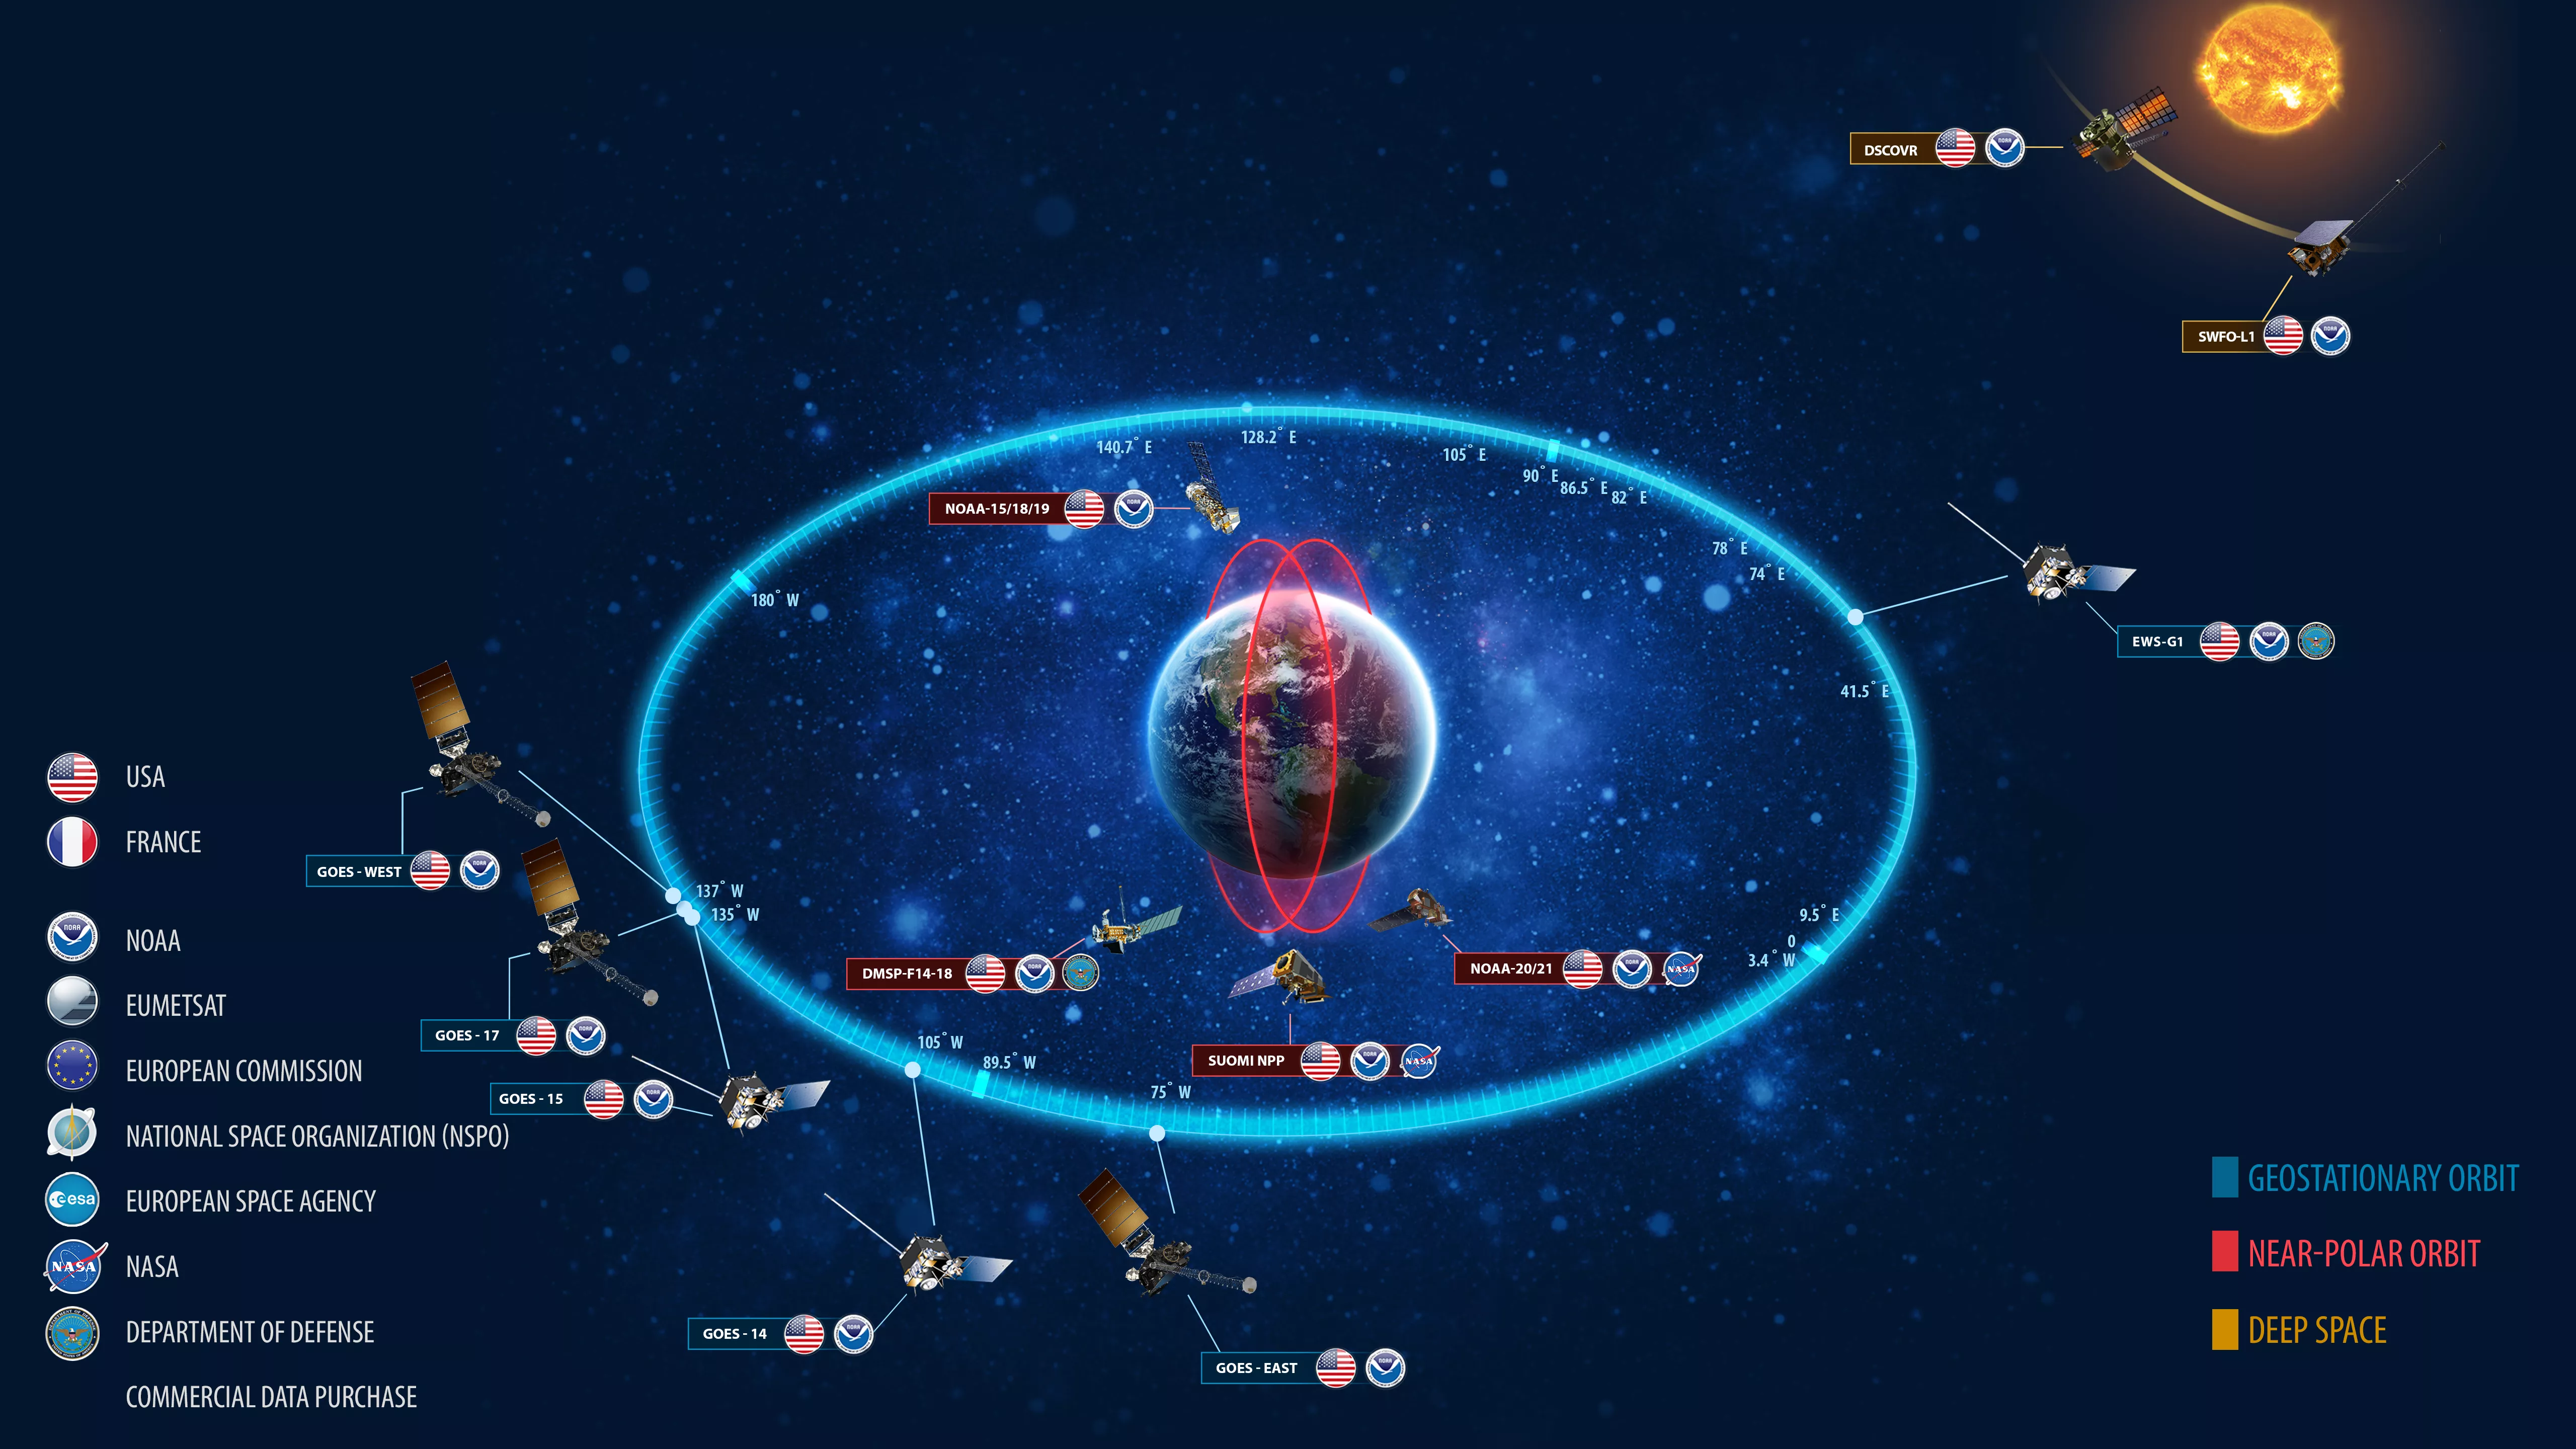
\includegraphics[width=\textwidth]{Figures/0. General/2023-03_NOAA-Observing-System.png}
        \caption{Imagen tomada de \url{https://www.nesdis.noaa.gov/current-satellite-missions/currently-flying}}
        \label{fig: NOAA sattelite 1}
    \end{subfigure}
    \hfill
\end{figure}


\textbf{Objetivo:} Describir una de las aplicaciones del uso de ondas electromagnéticas. En particular, explicar la transmisión de una señal electromagnética desde su generación en un satélite de toma de imágenes, pasando por su transmisión, llegado a la detección de esta por la antena y su conversión a una imagen.

\subsection{Introducción: Onda electromagnética}
\begin{itemize}
    \item ¿Qué es una onda electromagnética?
    \item Introducción al campo magnético
    \item Relación entre campo eléctrico y magnético
    \item Espectro electromagnético (Frecuencia y longitud de onda)
\end{itemize}

\subsection{Satélites y generación de señal}
\begin{itemize}
    \item ¿Qué es un satélite?
    \item Tipos de órbitas
          \begin{itemize}
              \item \url{https://scijinks.gov/orbit/}
          \end{itemize}
    \item Satélites NOAA: Un poco de la historia y su propósito.
          \begin{itemize}
              \item \url{https://www.n2yo.com/}
              \item \url{http://gpredict.oz9aec.net/}
          \end{itemize}
    \item Toma de “fotos” en un satélite
    \item Transformación de “fotos” a ondas (¿Qué propiedades de una onda transmiten información?)
          \begin{itemize}
              \item \url{https://www.goes-r.gov/featureStories/transformingEnergy.html}
          \end{itemize}
    \item Mostrar ejemplos de imágenes tomadas por los satélites NOAA.
\end{itemize}

\subsection{Transmisión de la señal e interferencia}
\begin{itemize}
    \item ¿Cómo viaja la onda a través de la atmósfera?
    \item Polarización de onda e importancia
    \item Modulación de onda estéreo FM
    \item Reflexión y difracción de la señal
    \item Ruido y pérdida de señal
\end{itemize}

\subsection{Antenas}
\begin{itemize}
    \item ¿Qué es una antena?
    \item Tipos de antenas y componentes esenciales
          \begin{itemize}
              \item Dipolos y dipolos dobles
              \item Antenas molinetes
          \end{itemize}
    \item Introducción a la transformada rápida de Fourier y su variante la transformada de Hilbert.
    \item Explicación de cómo las anteriores sirven para decodificar la señal.
          \begin{itemize}
              \item \url{https://gqrx.dk/}
          \end{itemize}
\end{itemize}

\subsection{Demostración}
\begin{itemize}
    \item Mostrar ejemplos de imágenes tomadas por los satélites NOAA.
    \item Si es posible hacer la demostración del recibimiento de una señal de los satélites NOAA.
    \item Acá dependemos un poco de la llegada de una antena pedida a través de internet.
    \item En caso tal de que no se pueda realizar la demostración en vivo, se mostrarán varios recursos de ejemplos reales que compañeros han realizado previamente.
\end{itemize}

\subsection{Actividad grupal}
\begin{itemize}
    \item Para la actividad grupal se usará la siguiente aplicación creada por los integrantes del equipo:
          \begin{itemize}
              \item \url{https://expofisica.grisu.co/}
          \end{itemize}
    \item El código de la aplicación se encuentra en el siguiente link de GitHub
          \begin{itemize}
              \item \url{https://github.com/Youngermaster/EAFIT-Notes/tree/main/LaTex/12th-Semester/Physics-II/path-connect}
          \end{itemize}

\end{itemize}

\section{Referencias y recursos que utilizaremos}
\begin{itemize}
    \item Software para mostrar durante la presentación: \url{https://gqrx.dk/}, \url{http://gpredict.oz9aec.net/}
    \item Páginas para mostrar durante la presentación: \url{https://scijinks.gov/orbit/}, \url{https://www.n2yo.com/}
    \item Referencias: \url{https://www.goes-r.gov/featureStories/transformingEnergy.html}
    \item How to Pull Images from Satellites in Orbit (NOAA 15,18,19 and METEOR M2): \url{https://www.youtube.com/watch?v=cjClTnZ4Xh4}
\end{itemize}

